\subsubsection{Batterie Management}
\label{subsubsec:batterie-management}
% Cleveres System
% BMS über MQTT Monitoren
% Was wird angezeigt
% Wie werden Daten interpretiert?
% Wie herausgefunden?

Der Herstellerdokumentation und Werbung ist an einigen Stellen zu entnehmen, dass im \gls{go1} ein intelligentes \gls{bms} verbaut ist.
Dieses ermöglicht es Nutzern, in Echtzeit Informationen zum Stand der Batterie abzugreifen und gegebenenfalls auf die Informationen
zu reagieren.
In der Herstellerdokumentation des Roboters ist nicht dokumentiert, wie die Daten erfasst oder interpretiert werden können,
es wird lediglich auf die beiden Übersichten in der mobilen Anwendung und der Webseite verwiesen, die in Abbildung \ref{fig:bms-app-web}
dargestellt werden.

\begin{figure}[h]
    \frame{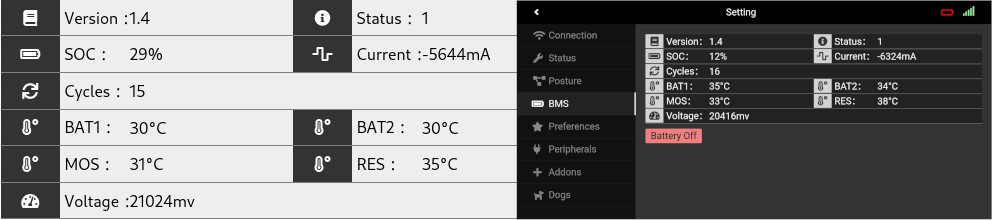
\includegraphics[width=\linewidth]{img/analyse/bms-app-web}}
    \caption{Batterieinformationen in der Webseite (links) und App (rechts)}\label{fig:bms-app-web}
\end{figure}

Die Ausgabe des MQTT-Explorers aus Kapitel \ref{subsubsec:led} beinhaltet ein Topic namens \texttt{bms/\allowbreak state}.
Auch die Prüfung der Webseite über die Entwicklertools innerhalb moderner Browser weisen auf die Bereitstellung der
\gls{bms} Daten über MQTT hin.
Der Dateipfad \texttt{src/\allowbreak plugins/\allowbreak mqtt/\allowbreak receivers/\allowbreak bms\allowbreak Receivers\allowbreak .ts}
und das konfigurierte MQTT-Topic \texttt{bms\allowbreak /state} bestätigen dies.
Gibt man nun die Message-Payloads des Topics aus, so erhält man folgendes Ausgabeformat.

\begin{lstlisting}
mosquitto_sub -h 192.168.123.161 -t bms/state -F %x
0104011bf5e8ffff0f001e1e1f23800da00d20002000a00da00da00d20002000800d
\end{lstlisting}

Man kann über die Entwicklertools der modernen Browser die Struktur der Daten zurückverfolgen.
Zeile \num{14} zeigt die Umwandlung der Message-Payload aus einem \texttt{Byte\allowbreak Buffer} in ein \texttt{Uint8Array}.
Laut der JavaScript-Dokumentation ist ein \texttt{Uint8Array} ein Array aus \num{8}-bit unsigned Integer\footcite{uint8array}.
Somit können je zwei Ziffern der hexadezimalen Ausgabe des \gls{bms} als ein Wert des Arrays interpretiert werden.
Die Zeilen \num{14} bis \num{17} und Zeile \num{20} in Listing \ref{lst:bms-reverse} zeigen die Umwandlungen der \num{8}-bit Integer.

\begin{lstlisting}[language=JavaScript,numbers=left,xleftmargin=2.5em,framexleftmargin=2em,firstnumber=14,label={lst:bms-reverse}]
const uint8s = new Uint8Array(message);
data.bms.version = uint8s[0] + "." + uint8s[1];
data.bms.status = uint8s[2];
data.bms.soc = uint8s[3];
data.bms.current = dataView.getInt32(4, true);
data.bms.cycle = dataView.getUint16(8, true);
data.bms.temps = [uint8s[10],uint8s[11],uint8s[12],uint8s[13]];
for (let i = 0; i < 10; i++) {
  data.bms.cellVoltages[i] = dataView.getUint16(14+i*2, true);
}
data.bms.voltage = data.bms.cellVoltages.reduce((a,c) => a+c);
\end{lstlisting}

\noindent Die Dokumentation der Klasse \texttt{DataView} zeigt, das die Funktionen \texttt{getInt32()} und \texttt{getUint16()}
folgenden Syntax haben\footcite{dataview}.

\begin{lstlisting}[language=JavaScript]
getInt32(byteOffset, littleEndian)
getUint16(byteOffset, littleEndian)
\end{lstlisting}

Somit wird in Zeile \num{18} ein \num{4}-Byte Integer ab dem fünften Byte der Message-Payload ausgelesen, in den Zeile
\num{19} ein \num{2}-Byte Integer ab dem neunten Byte und zehn weitere ab dem fünfzehnten Byte der Payload gelesen.
Die zehn letzten \num{2}-Byte Integer werden zu einer Gesamtzahl addiert.
Durch die Auswertungen der Webseite ergibt sich folgender Überblick über das Format der Payload.
Das verwendete Beispiel ist die oben gezeigte Ausgabe des Befehls \texttt{mosquitto\_\allowbreak sub}.

\begin{table}[h]
    \centering
    \begin{tabular}{|c|c|c|c|cc|}
        \hline
        \textbf{Byte} & \textbf{Format} & \textbf{Inhalt} & \textbf{Beispiel} & \multicolumn{2}{c|}{\textbf{Konvertierung}} \\ \hline
        0-1 & 2 x uint8 & Version & 01, 04 & \multicolumn{2}{c|}{v1.4} \\ \hline
        2 & uint8 & Status & 01 & \multicolumn{2}{c|}{1} \\ \hline
        3 & uint8 & State of Charge & 1b & \multicolumn{2}{c|}{27 \%} \\ \hline
        4-7 & int32 & Strom & f5e8ffff & \multicolumn{2}{c|}{-5899 mA} \\ \hline
        8-9 & uint16 & Zyklus & 0f00 & \multicolumn{2}{c|}{15} \\ \hline
        10-13 & 4 x uint8 & Temperaturen & \begin{tabular}[c]{@{}c@{}}1e, 1e,\\ 1f, 23\end{tabular} & \multicolumn{2}{c|}{\begin{tabular}[c]{@{}c@{}}30 \textdegree C, 30 \textdegree C\\ 31 \textdegree C, 35 \textdegree C\end{tabular}} \\ \hline
        14-33 & 10 x uint16 & Zell-Spannung & \begin{tabular}[c]{@{}c@{}}800d, a00d,\\ 2000, 2000,\\ a00d, a00d,\\ a00d, 2000,\\ 2000, 800d\end{tabular} & \multicolumn{1}{c|}{\begin{tabular}[c]{@{}c@{}}3456 mV, 3488 mV,\\ 32 mV, 32 mV,\\ 3488 mV, 3488 mV,\\ 3488 mV, 32 mV,\\ 32 mV, 3456 mV\end{tabular}} & \begin{tabular}[c]{@{}c@{}}\textbf{Summe:}\\ 20,992 V\end{tabular} \\ \hline
    \end{tabular}
    \label{tab:bms-format-matrix}
\end{table}

Im Kapitel \ref{sec:funktionserweiterungen-und-integration} wird gezeigt, wie die Informationen des \gls{bms} sinnvoll
ausgelesen und verwertet werden können.

